\documentclass[../main]{subfiles}
\begin{document}

\section{
  Brainfuck parsing and code generation
}

Now that we introduced the various techniques to generate programs from
pointer trees generated by \gls{constexpr} functions, we will use them in the
context of compile-time parsing and code generation for the Brainfuck language.
Therefore use data structures and code generation techniques introduced in
subsection \ref{lbl:ptr-tree-codegen}.

\subsection{
  Constexpr Brainfuck parser and AST
}

\subsubsection{
  AST
}

The Brainfuck \gls{ast} is defined in the header shown in appendix \ref{app:bf-ast}.
The header file also contains helper function definitions to handle \gls{ast} nodes
safely, such as \lstinline{visit} which will be used in one of the
code generation backends.

Here are the main data types:

\begin{itemize}
\item
\lstinline{node_interface_t}, which is a common base type for all \gls{ast} nodes.

\item
\lstinline{ast_token_t}, which represents a single \gls{ast} token.

\item
\lstinline{ast_block_t}, which represents an \gls{ast} block, which simply is a
\lstinline{std::vector} of \lstinline{std::unique_ptr<node_interface_t>}.

\item
\lstinline{ast_while_t}, which represents a while conditional block.
The instruction block itself is contained in an \lstinline{ast_block_t} value.

\end{itemize}

The implementation of the \gls{ast} are available in appendix \ref{app:bf-ast}
where you can observe that all the types are implemented as they would be
for a regular Brainfuck parser, except all their methods are \gls{constexpr}.

\begin{lstlisting}[
  language=c++,
  caption=Definition of the \gls{ast} visitor function,
  label=lst:bf-ast-visit-def
]{}
template <typename F>
constexpr auto visit(F f, ast_node_ptr_t const &p) {
  switch (p->get_kind()) {
  case ast_token_v:
    return f(static_cast<ast_token_t const &>(*p));
  case ast_block_v:
    return f(static_cast<ast_block_t const &>(*p));
  case ast_while_v:
    return f(static_cast<ast_while_t const &>(*p));
  }
}
\end{lstlisting}

The \lstinline{visit} function implementation also looks like a regular \cpp
function as shown in listing \ref{lst:bf-ast-visit-def}.
It is a higher order function that allows recursive operations on the \gls{ast} to be
carried in a type-safe manner.

\subsubsection{
  Parser
}

The Brainfuck parser, again, looks like nothing special. For that reason I will
not get into the implementation details. The function definition is available
in appendix \ref{app:bf-parser}.

On the surface: the parser takes a pair of begin and end iterators as an input.
It parses Brainfuck tokens until it reaches the end iterator or a while end
token, and returns a pair containing an iteretor pointing after the last parsed
token and the parsing result.

When a while begin token is reached, it calls itself recursively and resumes
parsing at the position of the iterator returned by the callee, which is right
after the while block.

The main parsing function implementation (including the function prototype)
is very condensed: it fits in 40 lines of code with a max line width set to 84.
It is no different from a regular Brainfuck parsing function except for it being
\gls{constexpr}, and it can actually be used as a regular \cpp program.

These make it much easier to debug as it can be ran through a \cpp debugger like
GDB or LLDB, and also more maintainable as it does not require any
template metaprogramming experience to understand the implementation.
Additionally, \gls{constexpr} execution enforces checks on memory allocations and
deallocations as well as memory bound checking. Therefore testing functions
in \gls{constexpr} contexts can help finding memory safety issues.

\subsection{
  A variety of techniques to generate code from a dynamic AST
}

Once the \gls{constexpr} parser is implemented, the next step consists in
figuring out how to transform its result, which contains dynamic memory,
into \cpp code.

As you may remember from subsection \ref{lbl:constexpr-programming},
there is no direct way to use values holding pointers to dynamic memory
directly as \glspl{nttp}.
Therefore it must be conveyed by other means or transformed into \glspl{litval}
to be used as template parameters for \cpp code generation.

I implemented several of these workarounds to compare them.
This will give us a clearer idea of their implementation difficulty,
and they will enable us to run compilation time benchmarks to compare their
compilation time performance.

\subsubsection{Pass-by-generator + ET}

The first technique I implemented was passing \gls{ast} nodes through lambdas
to convert them into expression templates.

\subsubsection{Pass-by-generator}

actually very hard to implement because \lstinline{std::unique_pointer}
lifetime management gets more difficult when combined with
\gls{constexpr} constraints.

% TODO: Mention compilation times

\subsubsection{Serializing the \gls{ast} into a \gls{litval}}

The last technique I will discuss, which is by far the most efficient
in regard to compilation time, consists in transforming the \gls{ast} into a
\gls{litval} that can be used as a \gls{nttp}.

As I've discussed in \ref{lbl:constexpr-programming}, a \gls{constexpr}
\lstinline{std::vector} return value can be transformed into a static array with
a trivial transformation. As long as a static array holds \glspl{litval},
the array itself remains a \gls{litval} as well, and can therefore be used
as a \gls{nttp}.

In order to do this, an intermediate serialized representation of the \gls{ast}
which must only contain \glspl{litval} must be implemented.
It is a fairly trivial task:

\begin{itemize}
\item
Polymorphism through the inheritance of \lstinline{node_interface_t}
can be replaced with the use of \lstinline{std::variant}, which is literal
as long as the value it holds is literal as well.

\item
Pointers contained in AST nodes can be replaced by integer indexes pointing to
internal values of the array (static or dynamic) in which serialized
AST nodes are stored.
\end{itemize}

\begin{lstlisting}[
  language=c++,
  caption=PBG intermediate representation type definitions,
  label=lst:flat-ir-typedef
]{}
/// Represents a single instruction token
struct flat_token_t {
  token_t token;
};

/// Block descriptor at the beginning of every block
/// of adjacent instructions.
struct flat_block_descriptor_t {
  size_t size;
};

/// Represents a while instruction, pointing to
/// another instruction block
struct flat_while_t {
  size_t block_begin;
};

/// Polymorphic representation of a node
using flat_node_t =
    std::variant<flat_token_t, flat_block_descriptor_t,
                 flat_while_t>;

/// AST container type
using flat_ast_t = std::vector<flat_node_t>;

/// NTTP-compatible AST container type
template <size_t N>
using fixed_flat_ast_t = std::array<flat_node_t, N>;
\end{lstlisting}

In listing \ref{lst:flat-ir-typedef}, I show how this was implemented in the
backend that will be used for the benchmarks.
Note that the serialized \gls{ast} can be stored either as a
\lstinline{flat_ast_t} for convenience in \glspl{consteval},
which can then be transformed into a \lstinline{fixed_flat_ast_t<N>}
to be passed as a \gls{nttp}.

In order

\begin{lstlisting}[
  language=c++,
  caption={\lstinline{block_gen} implementation},
  label=lst:flat-block_gen-impl
]{}
/// Support structure for generate_blocks function
struct block_gen_state_t {
  /// Flat AST blocks, result of block_gen
  std::vector<flat_ast_t> blocks;

  /// Keeping track of which block is being generated
  size_t block_pos = 0;

  /// Keeping track of the size of the AST
  size_t total_size = 0;
};

/// Extracts an AST into a vector of blocks of
/// contiguous operations
constexpr void block_gen(ast_node_ptr_t const &,
                         block_gen_state_t &);

/// block_gen for a single AST token. Basically just a
/// push_back.
constexpr void block_gen(ast_token_t const &tok,
                         block_gen_state_t &s) {
  s.blocks[s.block_pos].push_back(
      flat_token_t{tok.token});
}

/// block_gen for an AST block.
constexpr void block_gen(ast_block_t const &blo,
                         block_gen_state_t &s) {
  // Save & update block pos before adding a block
  size_t const previous_pos = s.block_pos;
  s.block_pos = s.blocks.size();
  s.blocks.emplace_back();

  // Preallocating
  s.blocks[s.block_pos].reserve(
      blo.content.size() + 1);
  s.total_size += blo.content.size() + 1;

  // Adding block descriptor as a prefix
  s.blocks[s.block_pos].push_back(
      flat_block_descriptor_t{
          blo.content.size()});

  // Flattening instructions
  for (ast_node_ptr_t const &node :
       blo.content) {
    block_gen(node, s);
  }

  // Restoring block pos after recursive block
  // processing
  s.block_pos = previous_pos;
}

/// block_gen for a while instruction.
constexpr void block_gen(ast_while_t const &whi,
                         block_gen_state_t &s) {
  s.blocks[s.block_pos].push_back(
      flat_while_t{s.blocks.size()});
  block_gen(whi.block, s);
}

constexpr void block_gen(ast_node_ptr_t const &p,
                         block_gen_state_t &s) {
  visit([&s](auto const &v) { block_gen(v, s); }, p);
}
\end{lstlisting}

Listing \ref{lst:flat-block_gen-impl} shows the implementation of the
\lstinline{block_gen} function. It is the first step of the overall
serialization process which transforms \lstinline{ast_block_t} values into
blocks of type \lstinline{flat_ast_t}.

The elements contained in these blocks have their indexes pointing to
the block indexes inside the \lstinline{blocks} member of the
\lstinline{block_gen_state_t} structure.

\begin{lstlisting}[
  language=c++,
  caption={\lstinline{flatten} function implementation},
  label=lst:flat-flatten-impl
]{}
constexpr flat_ast_t
flatten(ast_node_ptr_t const &p) {
  flat_ast_t result;

  // Extracting as vector of blocks
  block_gen_state_t block_gen_result;
  block_gen(p, block_gen_result);

  std::vector<flat_ast_t> const &semi_res =
      block_gen_result.blocks;
  result.reserve(block_gen_result.total_size);

  std::vector<size_t> block_map;
  block_map.reserve(semi_res.size());

  // Step 1: flattening

  for (flat_ast_t const &block : semi_res) {
    // Updating block_map
    block_map.push_back(result.size());

    // Flattening instructions
    std::copy(block.begin(), block.end(),
              std::back_inserter(result));
  }

  // Step 2: linking

  for (flat_node_t &current_node : result) {
    if (std::holds_alternative<flat_while_t>(
            current_node)) {
      flat_while_t &w_ref =
          std::get<flat_while_t>(current_node);
      w_ref.block_begin =
          block_map[w_ref.block_begin];
    }
  }

  return result;
}
\end{lstlisting}

The rest of the work consists in concatenate those blocks and replacing the
indexes to the blocks from the previous structure with indexes to the block
beginnings in its concatenated form. This work is carried out by the
function called \lstinline{flatten}, which is shown in listing
\ref{lst:flat-flatten-impl}.

Note that using \gls{constexpr} metaprogramming enables the use
of imperative programming, which is not possible using pure \gls{tmp} which
does not have mutable values.
Once we have parsing and serialization figured out, we only need to transform
the end result into a static array.

\begin{lstlisting}[
  language=c++,
  caption={\lstinline{parse_to_fixed_flat_ast} implementation},
  label=flat-parse_to_fixed_flat_ast-implementation
]{}
/// Parses a BF program into a fixed_flat_ast_t value.
template <auto const &ProgramString>
constexpr auto parse_to_fixed_flat_ast() {
  // Getting AST vector size into a constexpr variable
  constexpr size_t AstArraySize =
      flatten(parser::parse_ast(ProgramString))
          .size();

  // Initializing static size array
  fixed_flat_ast_t<AstArraySize> arr;
  std::ranges::copy(
      flatten(parser::parse_ast(ProgramString)),
      arr.begin());

  return arr;
}
\end{lstlisting}

Listing \ref{flat-parse_to_fixed_flat_ast-implementation} shows the
implementation of the final function that takes a string as a program
and transforms it into a \lstinline{fixed_flat_ast_t}, which can be used
directly as a \gls{nttp} and traversed trivially for code generation.

So far, this is the only function that takes a template parameter as an input,
and thus where the distinction between \gls{constexpr} programming and \gls{tmp}
begins.

\subsubsection{
  Difficulties
}

\begin{itemize}
\item Embedding text from the original string
\item \lstinline{if constexpr} requiring the definition of a \gls{constexpr} variable
\end{itemize}

\subsubsection{
  Implementation complexity
}

\subsubsection{
  Small synthetic variable-size benchmarks
}

We first begin by running two variable-sized benchmarks, consisting in
measuring compiler execution time as the \gls{ast} widens, and as the \gls{ast} deepens.

The first variable-sized benchmark consists in generating a valid BF \gls{ast} by
concatenating strings to generate a succession of BF while loops in a
\gls{constexpr} string. This benchmark was instantiated with sizes going from 1 to
10 with a step of 1, with 10 timing iterations for each size.

The second benchmark generates a string with
nested loops, making the \gls{ast} deeper as the benchmark size increases instead
of making it wider as in the previous case.

Both benchmarks generate programs of the same size so comparisons can be made
properly.

\begin{figure}
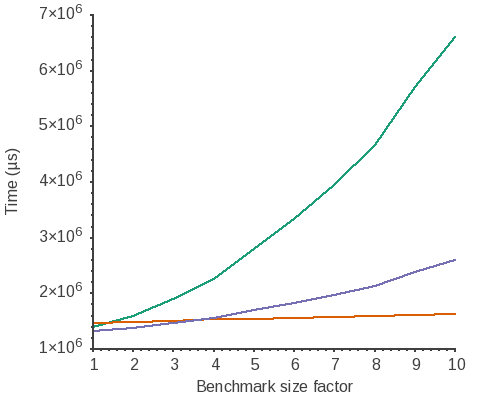
\includegraphics[scale=0.5]{images/bf-consecutive_loops.png}
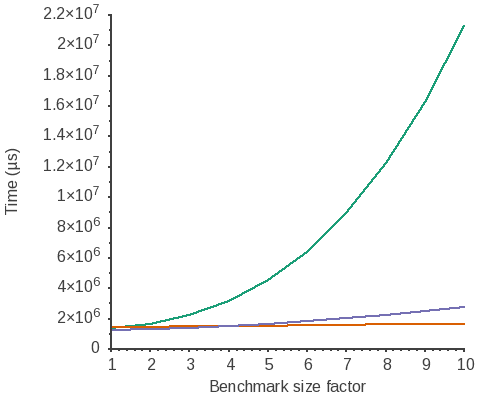
\includegraphics[scale=0.5]{images/bf-imbricated_loops.png}
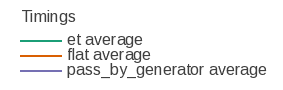
\includegraphics[scale=0.5]{images/bf-graph-legend.png}
\caption{
  Compiler execution time measurements for consecutive loops (left)
  and nested loops (right)
}\label{fig:bf-bench}
\end{figure}

Figure \ref{fig:bf-bench}
both highlight considerably higher compiler execution times for the expression
template based backend, high enough to suggest that the use of expression
templates induces an overhead higher than parsing and generating Brainfuck
programs using the \gls{pbg} backend. However the \gls{pbg}
backend still has a compile time overhead much higher than the flat backend,
which shows near constant compiler execution times on these small scale
benchmarks.

Finally, \gls{ast} deepening has a much higher impact on compile times than \gls{ast}
widening with the expression template backends, whereas the other backends seem
to scale similarly as the \gls{ast} grows wider or deeper.

\subsubsection{
  Large Brainfuck programs
}

The following benchmarks consist in measuring compiler execution times for
compiling Brainfuck code examples. These example programs are also used to
validate the metacompiler's backend implementations by compiling them and
verifying their output.

\begin{itemize}
\item A Hello World program (106 tokens).
\item The same Hello World program, ran twice (212 tokens).
\item A Mandelbrot set fractal viewer (11672 tokens).
\end{itemize}

\begin{figure}
\begin{tabular}{|c|c|c|c|}
\hline
Backend             & Hello World & Hello World x2  & Mandelbrot \\
\hline
Flat                & 1.81        & 2.25            & 49.68 \\
Pass-by-generator   & 9.77        & 34.37           & Failure (timeout) \\
Expression template & 50.60       & 192.73          & Failure (timeout) \\
\hline
\end{tabular}
\caption{BF compile time measurements in seconds
}\label{fig:BF-compile-times}
\end{figure}

The measurements in figure \ref{fig:BF-compile-times} help us better understand
how various metacompiling techniques behave at scale. The "Flat" backend shows
very good performance on all examples, including the Mandelbrot example that is
about 100 times larger than the Hello World example. However the other cases
highlight severe scaling issues and tend to confirm our previous hypothesis
being that using generator functions to pass values makes the code generation
quadratic. Finally, the \gls{et} backend performance highlights
heavy performance impact when expression templates are being used, which is
likely due to the complexity of the mechanisms expression templates involve like
\gls{sfinae} and overload resolution.

\subsubsection{
  Conclusions
}

\end{document}
